%%%%%%%%%%%%%%%%%%%%%%%%%%%%%%%%%%%%%%%%%%%%%%
%                insertmeeting
% 1) Title (something creative & funny?)
% 2) Date (MM/DD/YYYY)
% 3) Location (ex. Hagerty High School)
% 4) People/Committees Present 
% 5) Picture 
% 6) Start Time & Stop Time (ex. 12:30AM to 4:30PM)
%%%%%%%%%%%%%%%%%%%%%%%%%%%%%%%%%%%%%%%%%%%%%%
\insertmeeting 
  {New Year, New Intake} 
  {01/02/22} 
  {Hagerty High School}
  {Clayton, Nathan, Ritam}
  {Images/RobotPics/robot.jpg}
  {2:30 - 4:30}
  
\hhscommittee{Hardware}
\noindent\hfil\rule{\textwidth}{.4pt}\hfil
\subsubsection*{Goals}
\begin{itemize}
    \item redesign intake to function better with current robot
    \item Move servo to end of intake
    \item Replace hole for graphite pole with square attachment point for the current rev extrusion arm.

 

\end{itemize} 

\noindent\hfil\rule{\textwidth}{.4pt}\hfil

\subsubsection*{Accomplishments}
Hoping to get a new intake on the robot by our next meeting on the 8th, we started designing a slimmed down version of the intaek we tested at our last meeting. This new design uses a servo placed at the end of the arm. Although this is a worse way to make the intake function, it is a good quick solution that won’t have too many drawbacks at this competition. In an attempt to minimize the increase in weight from the servo, we designed this intake to be small and light. Another important part of this intake is that it connects to a REV extrusion instead of the graphite pole. Although the graphite is better than the REV extrusion, we don’t have enough time to remake the arm, then test it so make sure everything still runs correctly. This intake uses lots of pocketing to ensure the intake is as light as possible. It still will use a very similar system of O-ring belts attached to a roller and roller arm to suck in blocks, meaning the functionality should be nearly identical too. The final design also has a noticeably smaller footprint than the one before, because it no longer needs a set of pulleys to redirect a belt, like our previous design would have needed (Figure \ref{fig:010122_1})

\begin{figure}[htp]
\centering
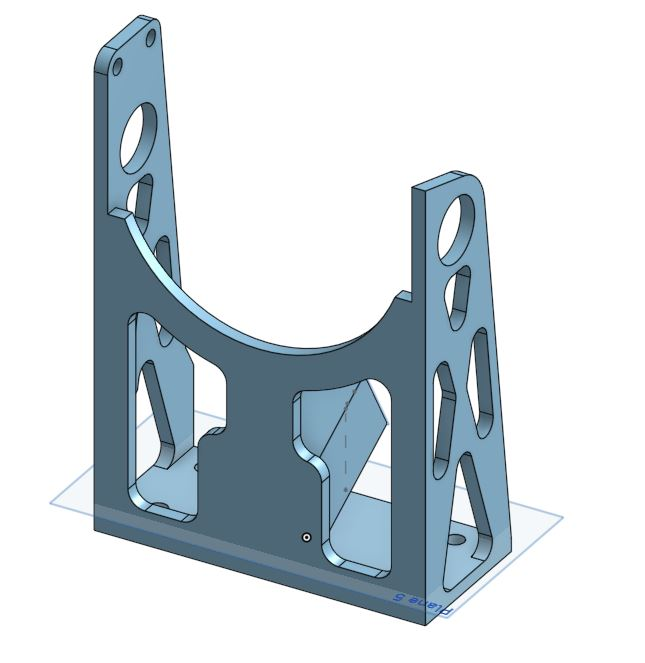
\includegraphics[width=0.95\textwidth, angle=0]{Meetings/January/01-02-22/1-2-22_CAD_Figure1 - Nathan Forrer.JPG}
\caption{Our new intake design}
\label{fig:010122_1}
\end{figure}


\whatsnext{
\begin{itemize}
    \item Print new roller intake
    \item Assemble and test new roller intake

\end{itemize} 
}

